\section{Результаты}
\subsection{Выбор метрики качества}
Для оценки результата использую метрики \texttt{accuracy} --- отношени верно классифицированных объектов к общему количеству объектов выборки. Для подбора параметров я использую кроссвалидацию по следующим параметрам:
\begin{lstlisting}[language=python, keepspaces=true]
params = {
    "dtc__max_depth": [None, 32, 16, 8],
    "dtc__min_samples_split": [2, 4, 8],
    "dtc__splitter": ["best", "random"],
    "dtc__criterion": ["gini", "entropy", "log_loss"],
}
\end{lstlisting}
Так как данных достаточно мало, то кроссвалидация разбивает выборку только на две части:
\begin{lstlisting}[language=python, keepspaces=true]
gscv_my_dtc = GridSearchCV(
      Pipeline([("dtc", MyDecisionTreeClassifier(classes=3))]),
      param_grid=params,
      cv=2,
      scoring="accuracy",
)
gscv_my_dtc.fit(train_X, train_y)
\end{lstlisting}
\pagebreak
\subsection{Точность на тестовой выборке}
\begin{center}
      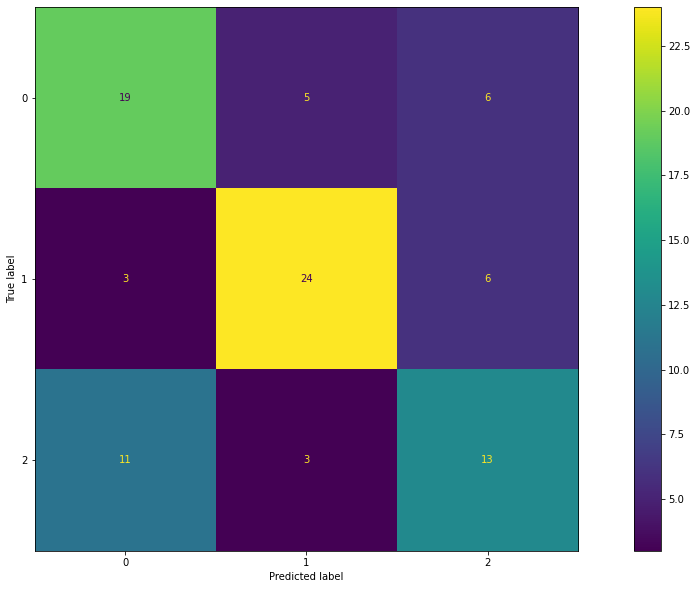
\includegraphics[width=\textwidth]{dtcmy.png}\newline\noindent
\end{center}
\begin{alltt}
      Лучшие гиперпараметры модели: \{
      'dtc__criterion': 'gini',
      'dtc__max_depth': None,
      'dtc__min_samples_split': 2,
      'dtc__splitter': 'best'
      \}
      Лучший счёт модели: 0.5377565752306823
      Метрика Accuracy: 0.6222222222222222
\end{alltt}
\pagebreak
\subsection{Дерево решений из sklearn}
\begin{center}
      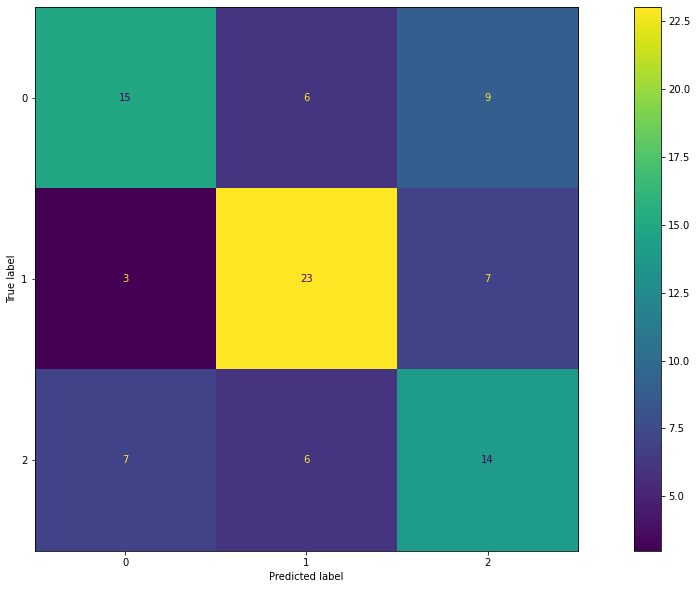
\includegraphics[width=\textwidth]{dtcsk.png}\newline\noindent
\end{center}
\begin{alltt}
      Лучшие гиперпараметры модели: \{
      'dtc__criterion': 'entropy',
      'dtc__max_depth': 8,
      'dtc__min_samples_split': 4,
      'dtc__splitter': 'best'
      \}
      Лучший счёт модели: 0.6133638817400038
      Метрика Accuracy: 0.5777777777777777
\end{alltt}
\pagebreak